\section{Specifications}
\label{sec:specs}
\newcounter{SpecID}

\subsection{Markers}
\refstepcounter{SpecID}
\label{spec:markers}

The arena, and tokens, are labelled with fiducial markers. Each
marker number is associated with a particular feature in the arena,
and also has an associated size.  The marker numbers and sizes are
as follows:

\begin{center}
\begin{tabular}{lcc}
  \toprule
  \textbf{Item} & \textbf{Marker Number} & \textbf{Marker Size (\si{mm})} \\
  \midrule
  Arena boundary & 0 -- 27 & 250 \\
  Central reservation & 28 -- 39 & 250  \\
  % 28 to 31 reserved for robot badges
  Tokens & 100 -- 199 & 80 \\
  \bottomrule
\end{tabular}
\end{center}

\subsection{Arena}
\refstepcounter{SpecID}
\label{spec:arena}

\begin{enumerate}
  \item The arena floor is an \SI{9}{m} $\times$ \SI{9}{m} rectangle. The
        tolerance of these two dimensions is $\pm$ \SI{250}{mm}.
  \item The floor of the arena is carpeted.
  \item The layout of the arena is given in Figure~\ref{fig:arena}. This
        figure is to scale.
  \item The outer walls of the arena are at least \SI{600}{mm} high, and the
        interior surface is white plastic-coated hardboard.
  \item Scoring zones will be bounded by metallic tape around the perimeter
        and internal boundaries. The inside edge of the tape marks the outside
        edge of the scoring zone.
  \item The raised area is \SI{2.4}{m} $\times$ \SI{2.4}{m} $\pm$ \SI{100}{mm},
        with a height of \SI{180}{mm} $\pm$ \SI{10}{mm}.
  \item The scoring zones extend a further \SI{2.4}{m} $\times$ \SI{2.4}{m} $\pm$ \SI{100}{mm}
        from the scoring zone, resulting in a total size of \SI{4.8}{m} $\times$ \SI{4.8}{m} $\pm$ \SI{200}{mm}.
  \item At the cardinal points of the arena are \SI{2.4}{m} $\times$ \SI{1.2}{m} $\pm$ \SI{100}{mm},
        raised at least \SI{180}{mm} $\pm$ \SI{10}{mm}.
  \item Scoring zones for teams will be offset 90\degree anti-clockwise, such
        that a team isn't directly in front of their own scoring zone.
  \item The starting location of the robots is given in Figure~\ref{fig:arena}.
        Teams are allowed to place their robot anywhere such that the entire
        robot is within \SI{1}{m} of the starting point, which will be
        indicated on the floor of the arena. The starting zones are along the
        shorter (\SI{8}{m}) walls of the arena.
\end{enumerate}

\begin{figure}
  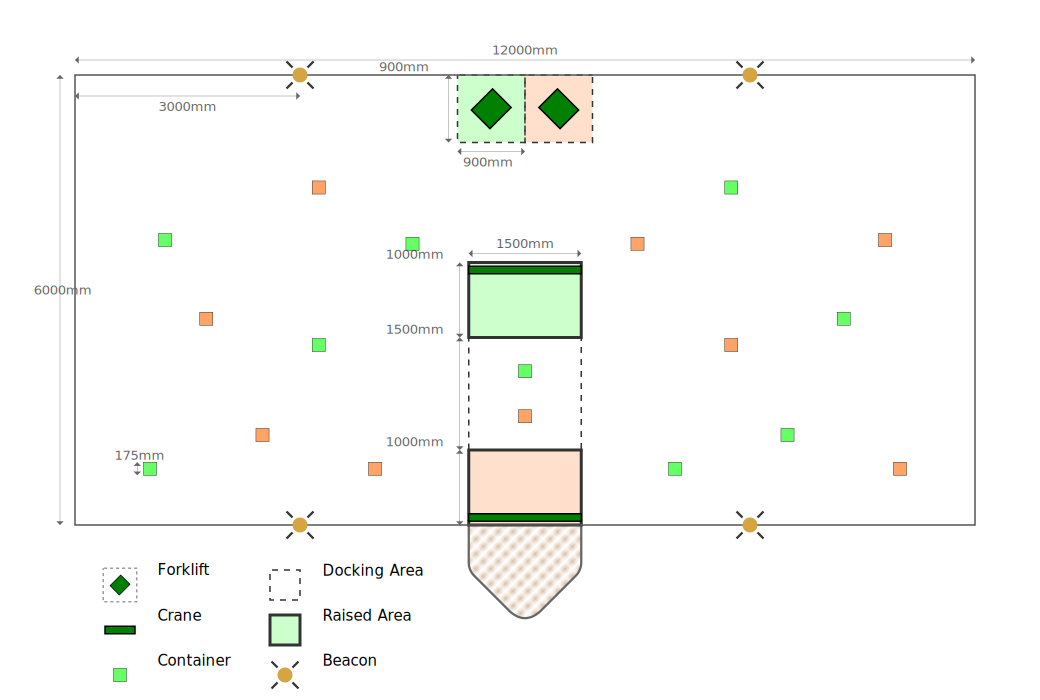
\includegraphics[scale=0.58]{fig-arena.pdf}
  \caption{Layout zones and tokens in the arena.}
  \label{fig:arena}
\end{figure}

\subsection{Tokens}
\refstepcounter{SpecID}
\label{spec:tokens}

\begin{enumerate}
  \item The tokens are \SI{100}{mm} $\times$ \SI{100}{mm} ($\pm$ \SI{10}{mm}).
  \item Tokens are placed in a pseudo-random, rotational-symmetrical pattern.
  \item Teams will start with 1 token directly in front of them, equidistant
        between their starting zone and the scoring zones.
  \item Tokens will start in the neutral area in the arena, with at least \SI{500}{mm}
        between the arena wall, scoring zones and tokens.
\end{enumerate}
